%This chapter/section is about the work on ``dc-smearing in GPP''
%Created by kp on Sep 17, 2011

\hspace{0.5cm}
% \newline \newline
%\newline  %double \newline gives underfull warnings

\begin{comment}
This is here just to remind me about this way of making comments
And, also to add some more reminders to myself.
1) change the figure size parameters to fit to the page if possible. 2) if related, put two or more figures side by side to save space as well as to make the organization better (otherwise, the compiler may put figures randomly and thus losing the sense of order/continuity)

It is assumed that the efficiency depends on the number of photoelectrons (the corresponding variable in the data ntuple is ``nphe''), which in turn is determined by the hit location on the Cerenkov PMT-projected plane (defined by the projected 
\th and \ph) as well as the angle with which the particle hit the plane. \ref{fig:genEvnts3}
\end{comment}

%%%%%%%%%%%%%%%%%%%
%   Note: The following section disabled because it is also in introChp4Sim.tex which includes this file with \input{filename}
%%%%%%%%%%%%%%%%%%%
%\section{GSIM POST PROCESSOR (GPP)}  
A lot of known, unknown, quantified, and unquantified factors such as temperature, alignment, dead channels, electronic malfunction etc affect the performance of the CLAS detector. But, GSIM does not include all these effects and, hence, the efficiency of the detector is always less than what the simulation provides us. To make the simulation more realistic by taking into account some of those effects, another CLAS software called GSIM Post Processor (GPP) is used to process the GSIM output. The GPP can change the DC, SC, CC and EC signals produced in the simulation. The DC signals can be changed by (a) accounting for the dead wires according to the calibration database, (b) shifting the DOCA mean value, and (3) smearing the hit signals according to the resolution determined by the calibration database or according to the command line input. Likewise, SC signals can be changed with a parameter input for smearing the time resolution. And, for the CC and EC signals, the GPP can use the hardware thresholds\cite{jxZhang_th}.

As the experimental conditions and detector configurations can change from one experiment to another, in order to run the GPP, we must have our own experiment specific calibration constants and parameters such as the run number (R), the DC smearing scale values for regions 1, 2 and 3 (a, b, c) and the SC smearing scale value (f). Even for a given experiment, these constants and parameters are determined to be different for different data sets (corresponding to a given beam energy, for example). The value for R can be any run number belonging to a specific data set. This number is used to identify the entry of the calibration constants in the database that corresponds to the given data set.  In order to simplify the job, we decided to use the timing resolutions determined by the calibration database assuming that they are good enough and need only to determine new values for the DC smearing. %(the reason to do this is that with the default (calibration database) resolution, the energy resolution in the data and the simulation seemed to differ significantly (as will be evident below when we compare the widths of the simulation & real data elastic peaks) 
To further simplify the job, we assumed that the three DC Regions had identical resolutions, so the DC smear parameters a, b, and c would have the same values, and the common DC-smear value is what is determined from the procedure described below.



%\subsection{\href{http://www.jlab.org/Hall-B/secure/eg4/adhikari/Analysis/SimStuffs/moniDcSmear.html}{Determining Dc-smear scales for GPP} to have the energy resolution of simulation comparable with that of the CLAS}
In order to determine the DC-smear, we generated a statistically significant number (about half million) of elastic-electron events distributed according to the elastic cross section and then ran them through GSIM, GPP and RECSIS. The pure proton target events, turning off the radiative effects are generated using the existing %Genova inherited 
STEG event generator. %As an example, the 2.3 GeV events looked like as shown in fig(\ref{fig:genEvnts3}) when histogrammed in the quantity $\Delta$E.

%(/w/hallb/claseg4/adhikari/GSIM_RECSIS/mod_osip_bost/mod_osip_bostVadim11_64tNH3). I modified the two files sgm_model.f & cor_peak_proton.f 
%which are kept for backup in the same directory where eps files are. In addition, the routines of bost.f were replaced with the latest 
%(/w/hallb/claseg4/adhikari/GSIM_RECSIS/bost09.f, soft linked by the old name bost.f), both generate_map and work directories use all these three files
% See my comments on cor_peak_proton.f at the very bottom of this file
\begin{comment} %Disabling this one to replace it with a figure that his a caption on the side rather than at the bottom.
\begin{figure}[h] %ht, htpb (p - float, b = bottom, h=? t = top)
  \leavevmode 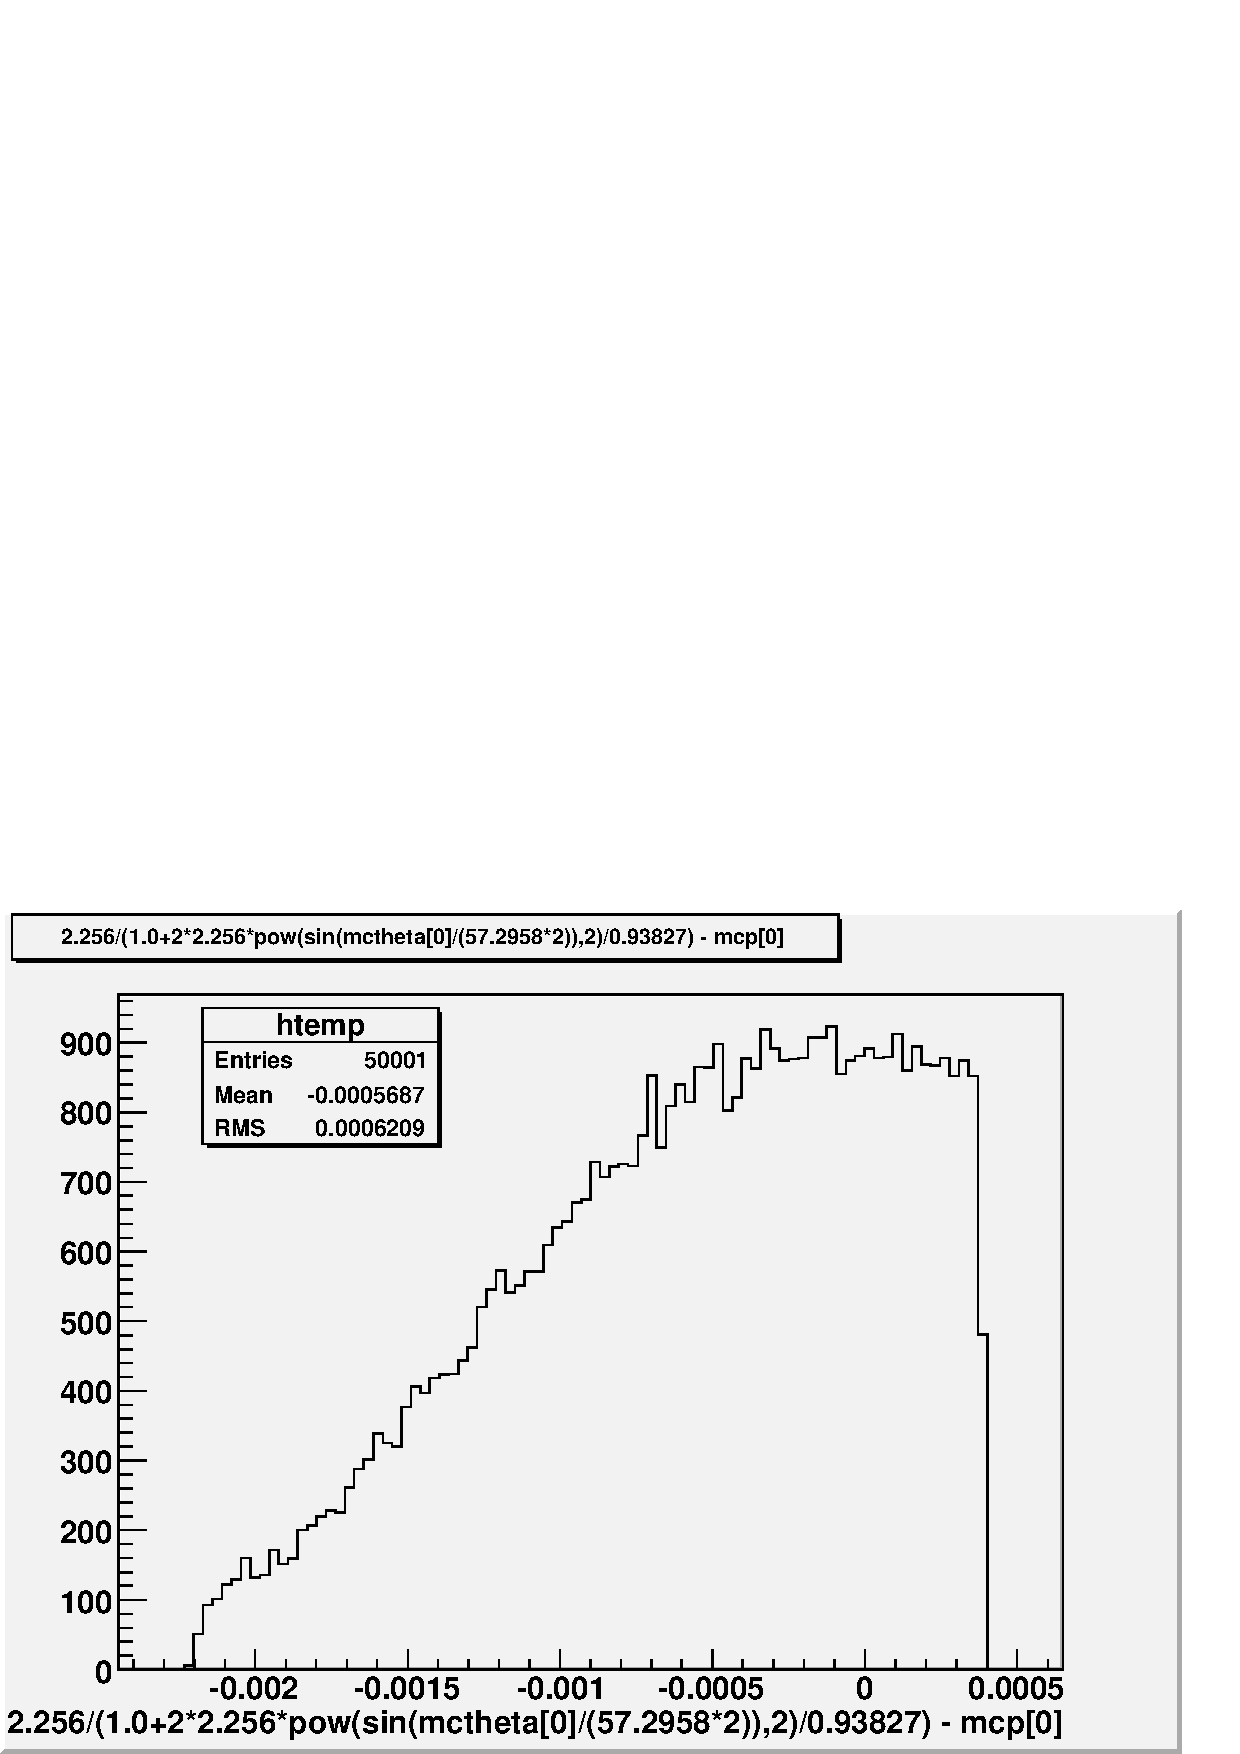
\includegraphics[width=0.6\textwidth]{figuresEG4/DcSmear/genEvntsElastOnlyEb3.png} 
  \caption[$\Delta$E of generated elastic events]{$\Delta$E of 2.3 GeV generated elastic-only proton-target events (no internal radiative effects).}
  \label{fig:genEvnts3}
\end{figure}



\begin{SCfigure} %http://en.wikibooks.org/wiki/LaTeX/Floats,_Figures_and_Captions (needs packages \usepackage[pdftex]{graphicx} & \usepackage{sidecap})
  \centering
  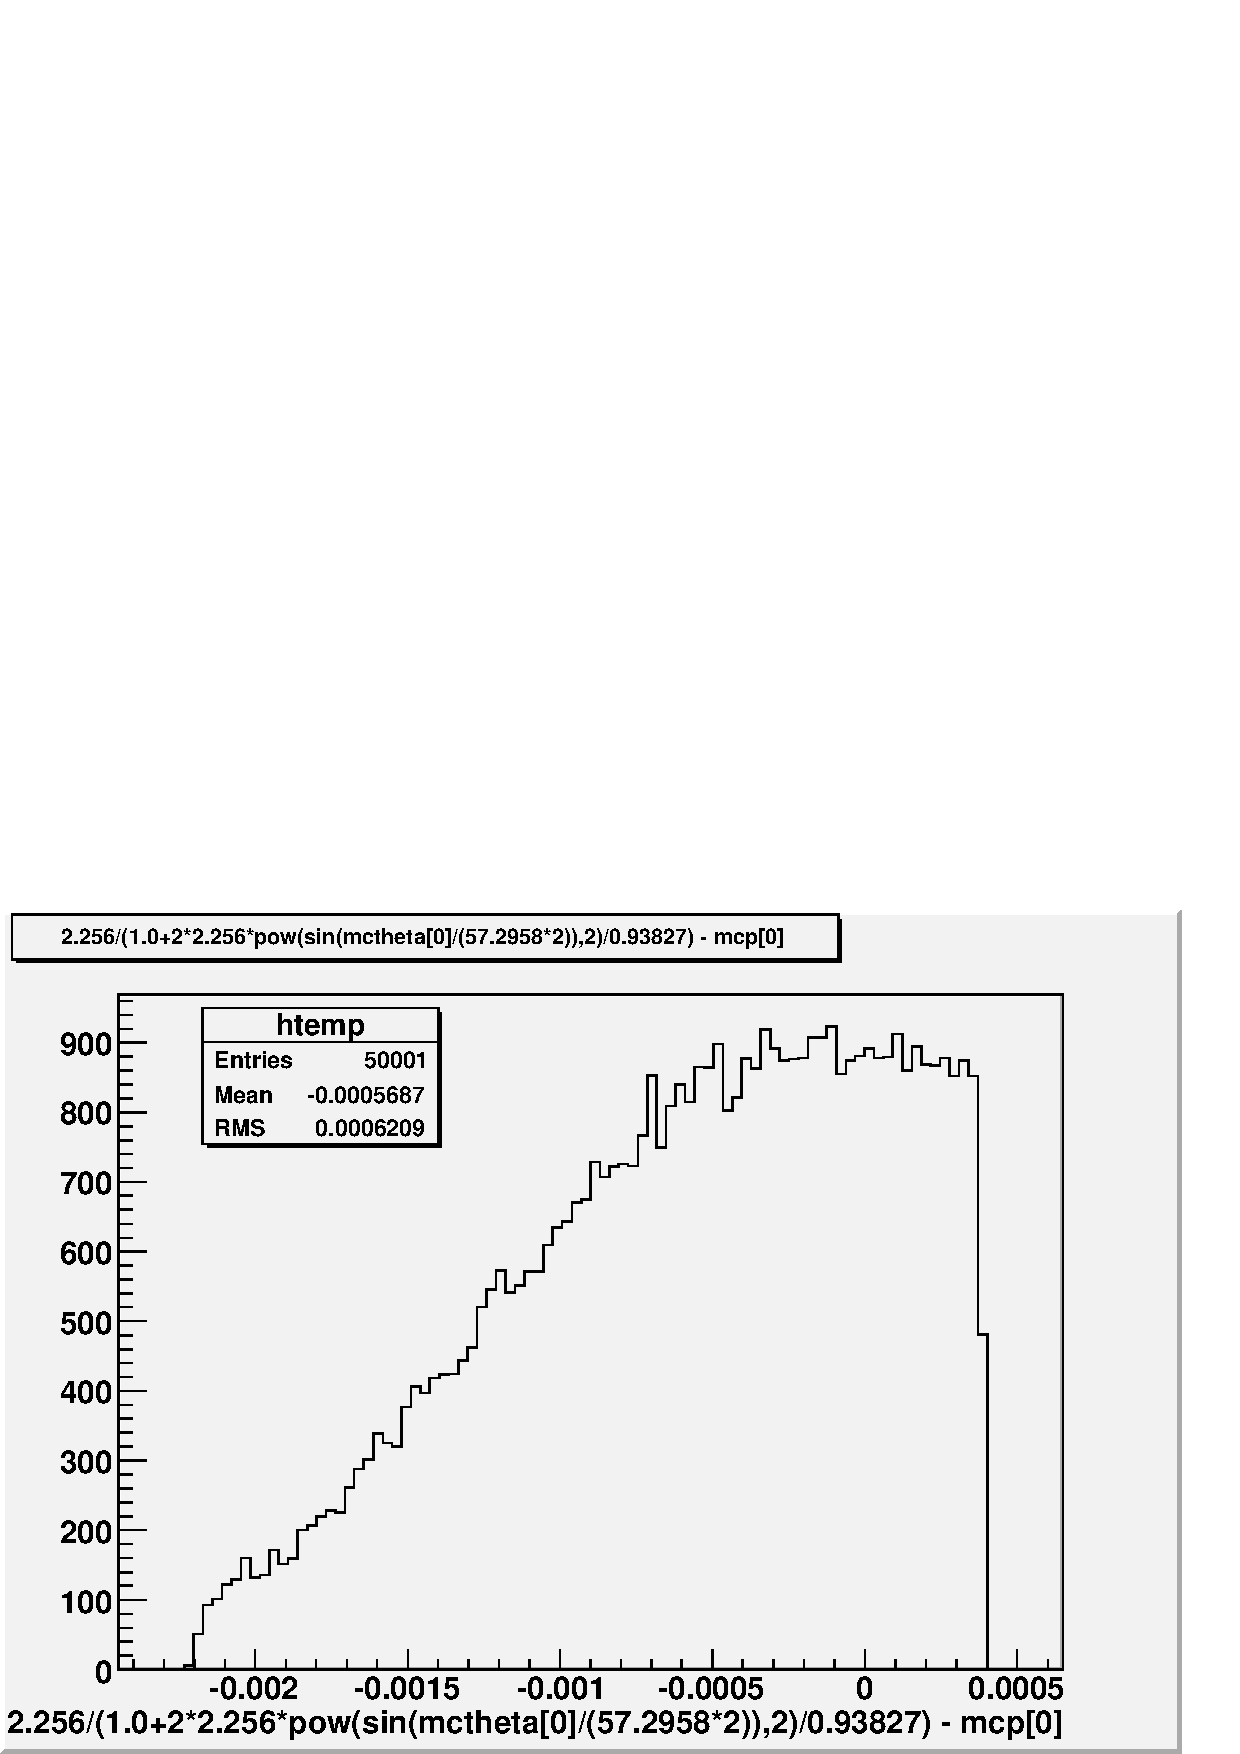
\includegraphics[width=0.7\textwidth]{figuresEG4/DcSmear/genEvntsElastOnlyEb3.png}
  \caption[$\Delta$E of generated elastic events]{$\Delta$E of 2.3 GeV generated elastic-only proton-target events (no internal radiative effects).}
  \label{fig:genEvnts3}
\end{SCfigure}

 \end{comment}

%\subsection{Finding the variation of the width of the simulated elastic peak as a function of DC-smear scale for GPP.}
The simulated elastic events are then fed into GSIM, GPP and RECSIS, with GSIM and RECSIS used in the same configuration as when processing the CLAS data 
during the ``pass-1'' phase, and GPP run with different values of DC-smear scales as inputs. The reconstructed data coming out of RECSIS corresponding to 
a given value of DC-smear is then histogrammed in $\Delta$E again and fitted to a Gaussian to get its $\sigma$ (characterizing width) of and mean 
(characterizing position). As we can see in figures \ref{fig:dcSm1.3} and \ref{fig:dcSm2.9}, %fig(\ref{fig:dcSmEff}), %This didn't give proper number
the width of the elastic peak increases with the DC-smear but the position stays more or less the same as expected. In fact, when the two are plotted 
against DC-smear (as in figures \ref{fig:SigmaVsm} and \ref{fig:MeanVsm}) %(as in fig (\ref{fig:ParsVsm})), %This didn't give proper number 
the width shows a linear dependance.



%Don't delete the following commented out lines. They are important reminders.
%The following four images are made using ~/Acceptance/SimStuffs/dE_resolHistoFits.C and enabling ``#define DRAW_EPS'' & ``#define USE_THETA_ALL''
\begin{comment} %=======================================Comments begin
%idea source: http://texblog.wordpress.com/2007/08/01/placing-figurestables-side-by-side-minipage/ : Placing figures/tables side-by-side (\minipage)
%This method of putting figures/tables side by side doesn't have the option of global caption (if there is, it treats it like a
% caption of a different figure assigning it with a different figure number in the output file. So, I chose the 'subfigure' method instead
\begin{figure}[h]
\begin{minipage}[b]{0.5\linewidth}
\centering
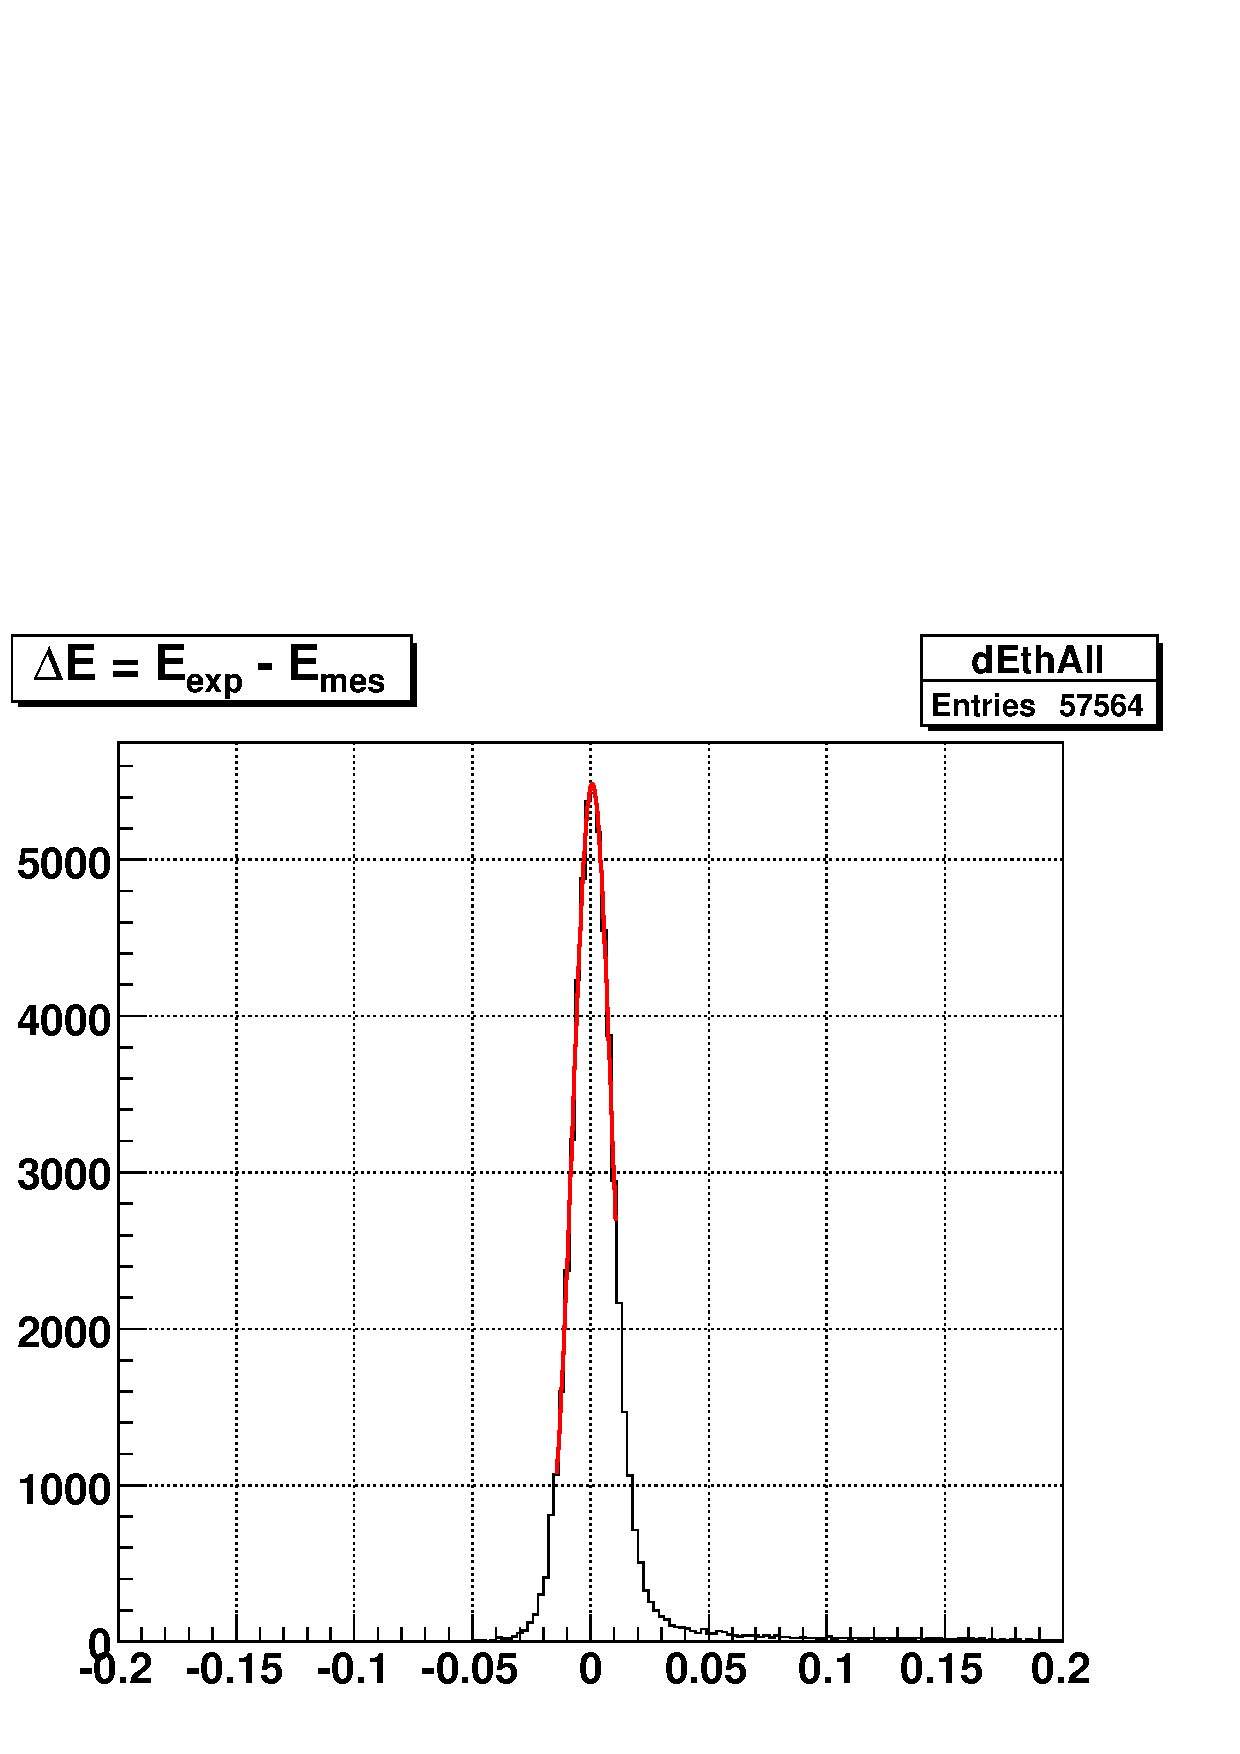
\includegraphics[scale=0.37]{figuresEG4/DcSmear/dE_ThAllEb3_DcSmear1.3.png}
\caption{$\Delta$E of 2.3 GeV simulated elastic-only proton-target events (see fig(\ref{fig:genEvnts3})) after passing through GSIM, GPP 
  (with Dc-smear scale of 1.3) and RECSIS.}
\label{fig:figure1}
\end{minipage}
\hspace{0.0cm} %\hspace{0.1cm}
\begin{minipage}[b]{0.5\linewidth}
\centering
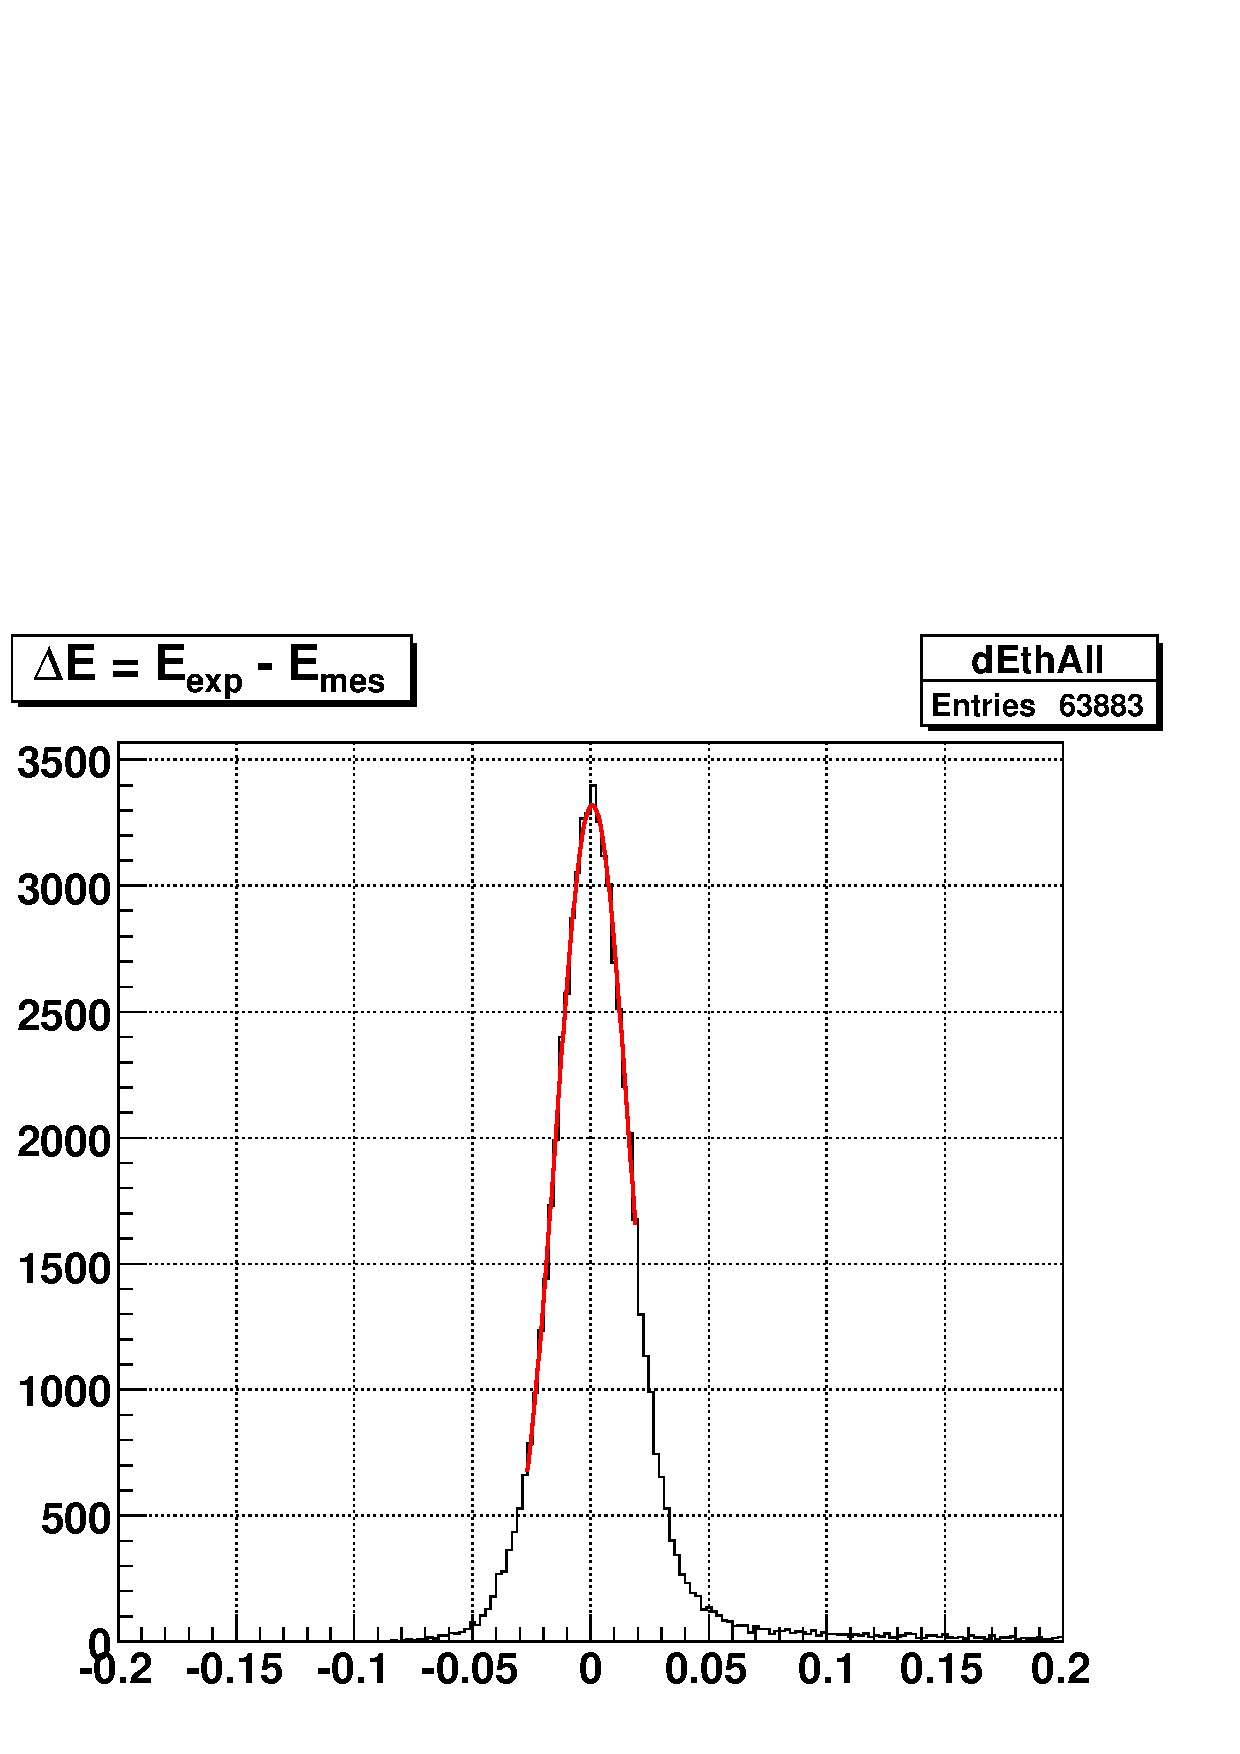
\includegraphics[scale=0.37]{figuresEG4/DcSmear/dE_ThAllEb3_DcSmear2.9.png}
\caption{$\Delta$E of 2.3 GeV simulated proton elastic-only events after passing through GSIM, GPP (with Dc-smear scale of 2.9) and RECSIS.}
\label{fig:figure2}
\end{minipage}
\caption{$\Delta$E of 2.3 GeV simulated elastic-only proton-target events (see fig(\ref{fig:genEvnts3})) after passing through GSIM, GPP (with Dc-smear scale of 1.3) and RECSIS.}
\end{figure}
\end{comment}  %=======================================Comments end


% idea source: http://texblog.wordpress.com/2007/08/28/placing-figurestables-side-by-side-subfigure/ :Placing figures/tables side-by-side (\subfigure)
% Can include any number of figures/tables, not just two.
\begin{figure}[H]
\centering
\subfigure[Dc-smear]{
\includegraphics[scale=0.32]{figuresEG4/DcSmear/dE_ThAllEb3_DcSmear1p3}%.png}
\label{fig:dcSm1.3}
}
\subfigure[Dc-smear]{
\includegraphics[scale=0.32]{figuresEG4/DcSmear/dE_ThAllEb3_DcSmear2p9}%.png}
\label{fig:dcSm2.9}
}
\label{fig:dcSmEff} %Effect of Dc-smear
%\caption[Optional caption for list of figures]{Caption of subfigures \subref{fig:subfig1}, \subref{fig:subfig2} and \subref{fig:subfig3}}
\caption[$\Delta$E of reconstructed simulated events]{$\Delta$E of 2.3 GeV simulated elastic-only proton-target events passing through GSIM, GPP (with two different Dc-smear scales), and RECSIS.}
\end{figure}




\begin{figure}[H]
\centering
\subfigure[$\sigma$ vs DC-smear]{
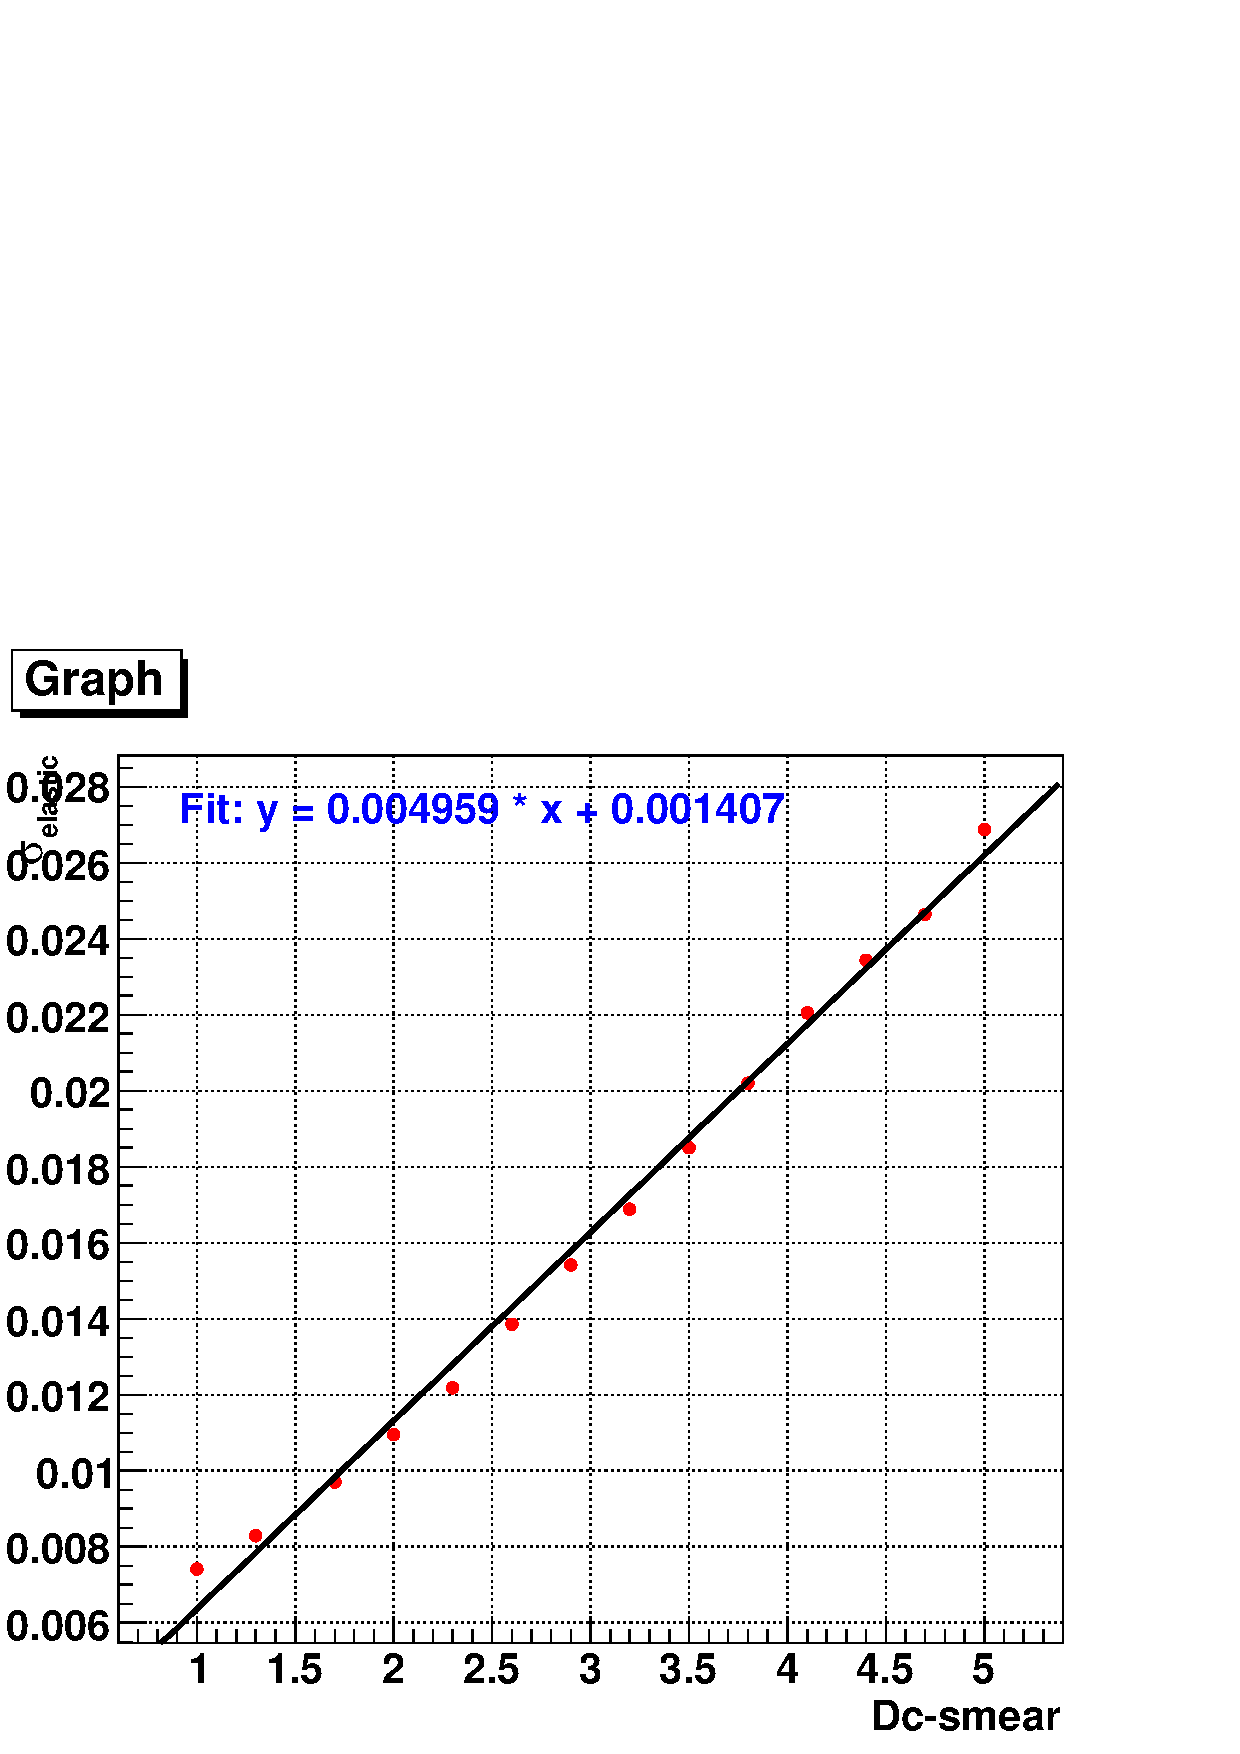
\includegraphics[scale=0.32]{figuresEG4/DcSmear/grSigmaVsDcSmear_Eb3.png}
\label{fig:SigmaVsm}
}
\subfigure[Mean vs DC-smear]{
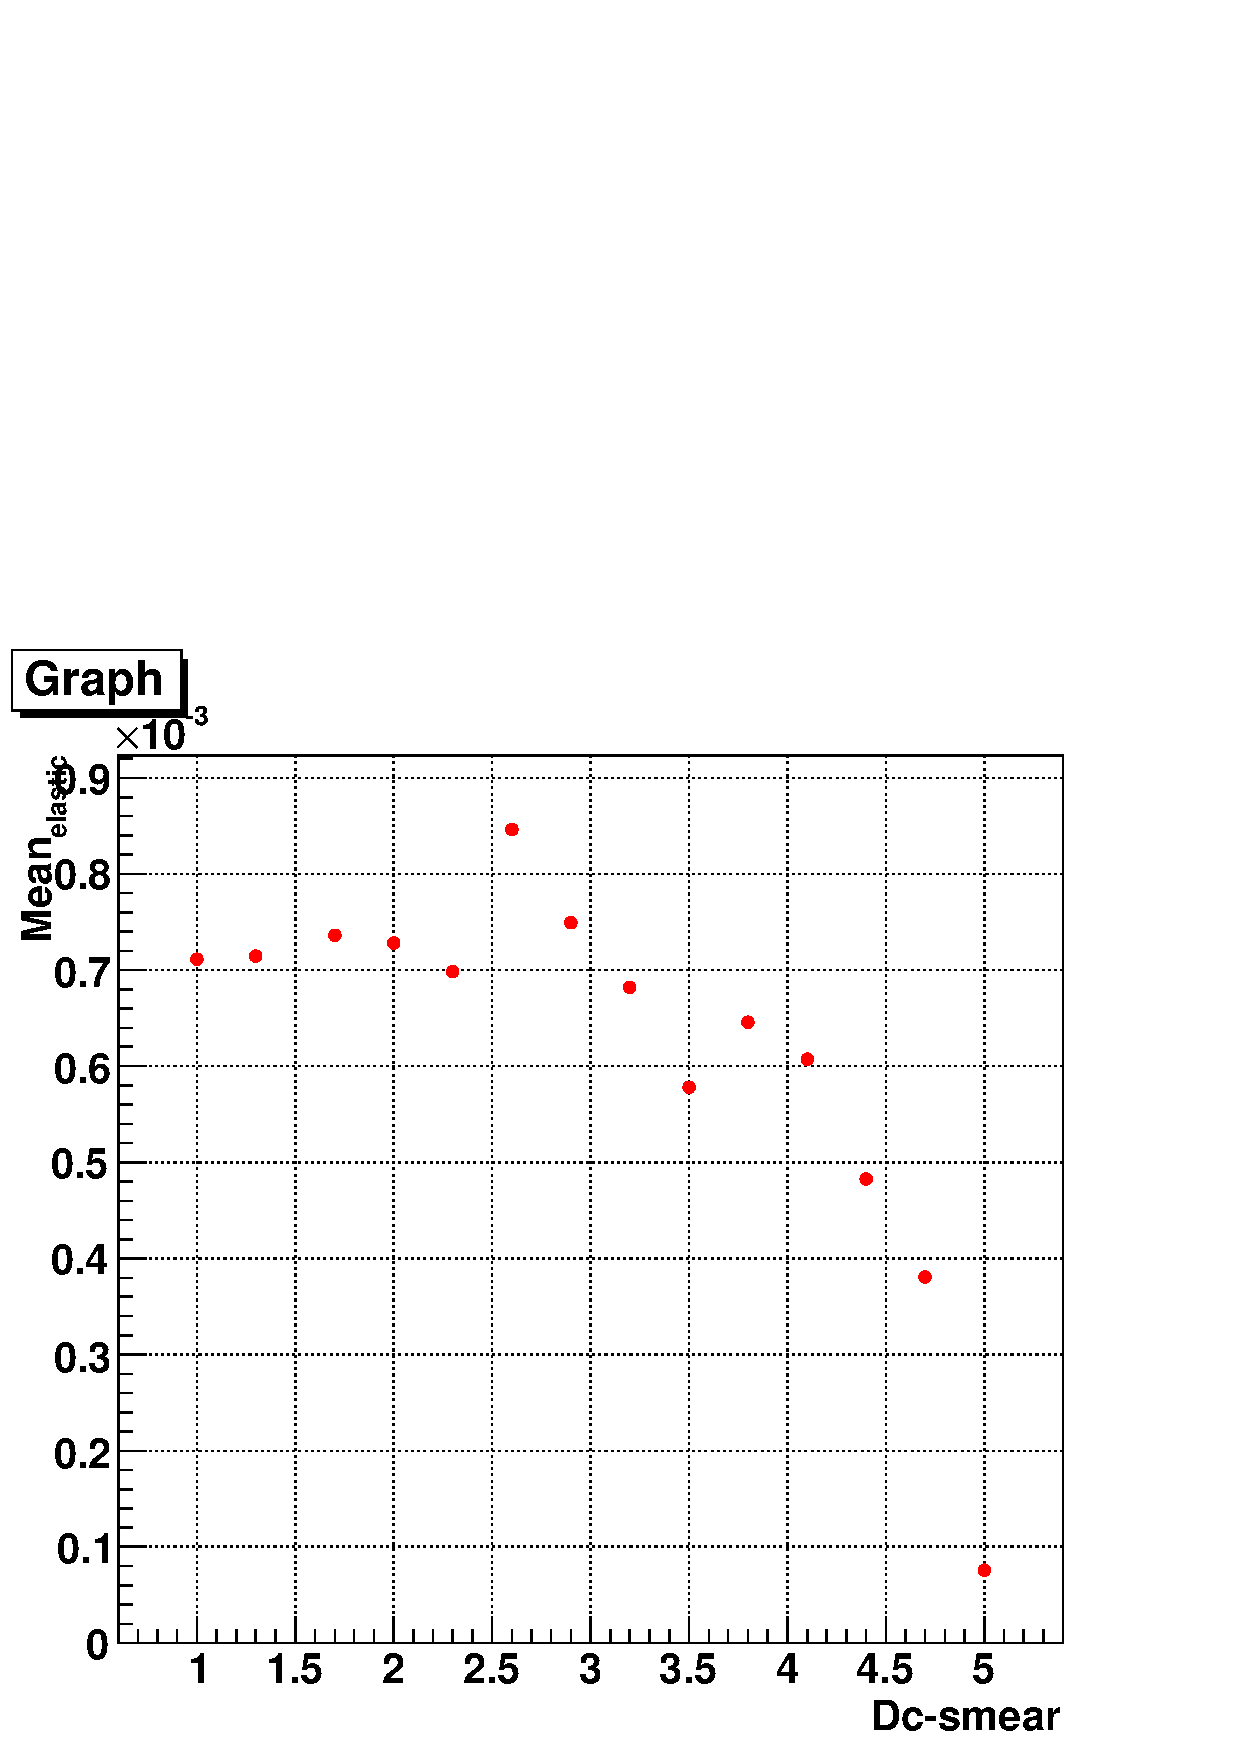
\includegraphics[scale=0.32]{figuresEG4/DcSmear/grMeanVsDcSmear_Eb3.png}
\label{fig:MeanVsm}
}
\label{fig:ParsVsm} %Effect of Dc-smear
%\caption[Optional caption for list of figures]{Caption of subfigures \subref{fig:subfig1}, \subref{fig:subfig2} and \subref{fig:subfig3}}
\caption[DC-smearing effects on elastic peak]{Graphs showing the dependence of width and position (obtained from the Gaussian fits as shown in the fig (\ref{fig:dcSmEff}) of the elastic peaks on the DC-smear applied to GPP.}
\end{figure}


\subsection{Finding the width of the real CLAS data elastic peak.}
With the knowledge of the DC-smear dependence of energy resolution (Fig. \ref{fig:SigmaVsm}), if we also know the resolution in the real data, 
we can determine the right value of DC-smear which would make the resolution in the simulation comparable with that in the real data. So, 
the next step is to find the resolution in the real CLAS data, which is done again by measuring the width of the elastic peak in the real data. 
But, because the real data is a very complex mixture of events coming from various reaction channels, we must first have a way to separate the elastic 
data from the rest. One method entails histogramming \dE from both the \nh3 and \c12 target data (for a given beam energy) and subtracting 
the latter (after the cross-normalization) from the former (as in fig (\ref{fig:elNH3mC})) to effectively remove the contribution from nitrogen 
component of the \nh3 target leaving the contribution coming only (mostly) 
%More words about this background subtraction can be found in the section for the inclusive momentum correction.
from the proton component. Another method consists of using only the \nh3 data but this time calculating the helicity dependent cross-section 
difference in the elastic region Fig. (\ref{fig:elXsDif}). In the latter method, the difference removes the contribution from the unpolarized 
nuclear background because they have the same contribution to the opposite helicity state cross-sections. After the elastic data is separated, its 
\dE distribution is fitted to a Gaussian as with the simulation data and we arrive at the experimental energy resolution. 
%Since on the simulation side, we used the total cross-section, to make an apple-to-apple comparison, the measurement coming from the 1st method
%would be better choice for the experimental data.

% Put a intra-thesis chapter/section link (rather than the web link) in thesis version
% \href{http://www.jlab.org/Hall-B/secure/eg4/ripani/Reference/Reference.html}{groups 1, 2 and 4 cuts}. 
% Check DoEvent..() function in file /u/home/adhikari/Acceptance/SimStuffs/dE_resol_DataSim.C to see what cuts were used to select the events


%The following image is made using ~/Acceptance/SimStuffs/subtractHistos4ProdElast.C and enabling ``#define DRAW_EPS'' & ``#define USE_THETA_ALL''
%The following four images are made using ~/Acceptance/SimStuffs/dE_resolHistoFits.C and enabling ``#define DRAW_EPS'' & ``#define USE_THETA_ALL''
\begin{figure}[h] %ht, htpb (p - float, b = bottom, h=? t = top)
\centering
  \leavevmode 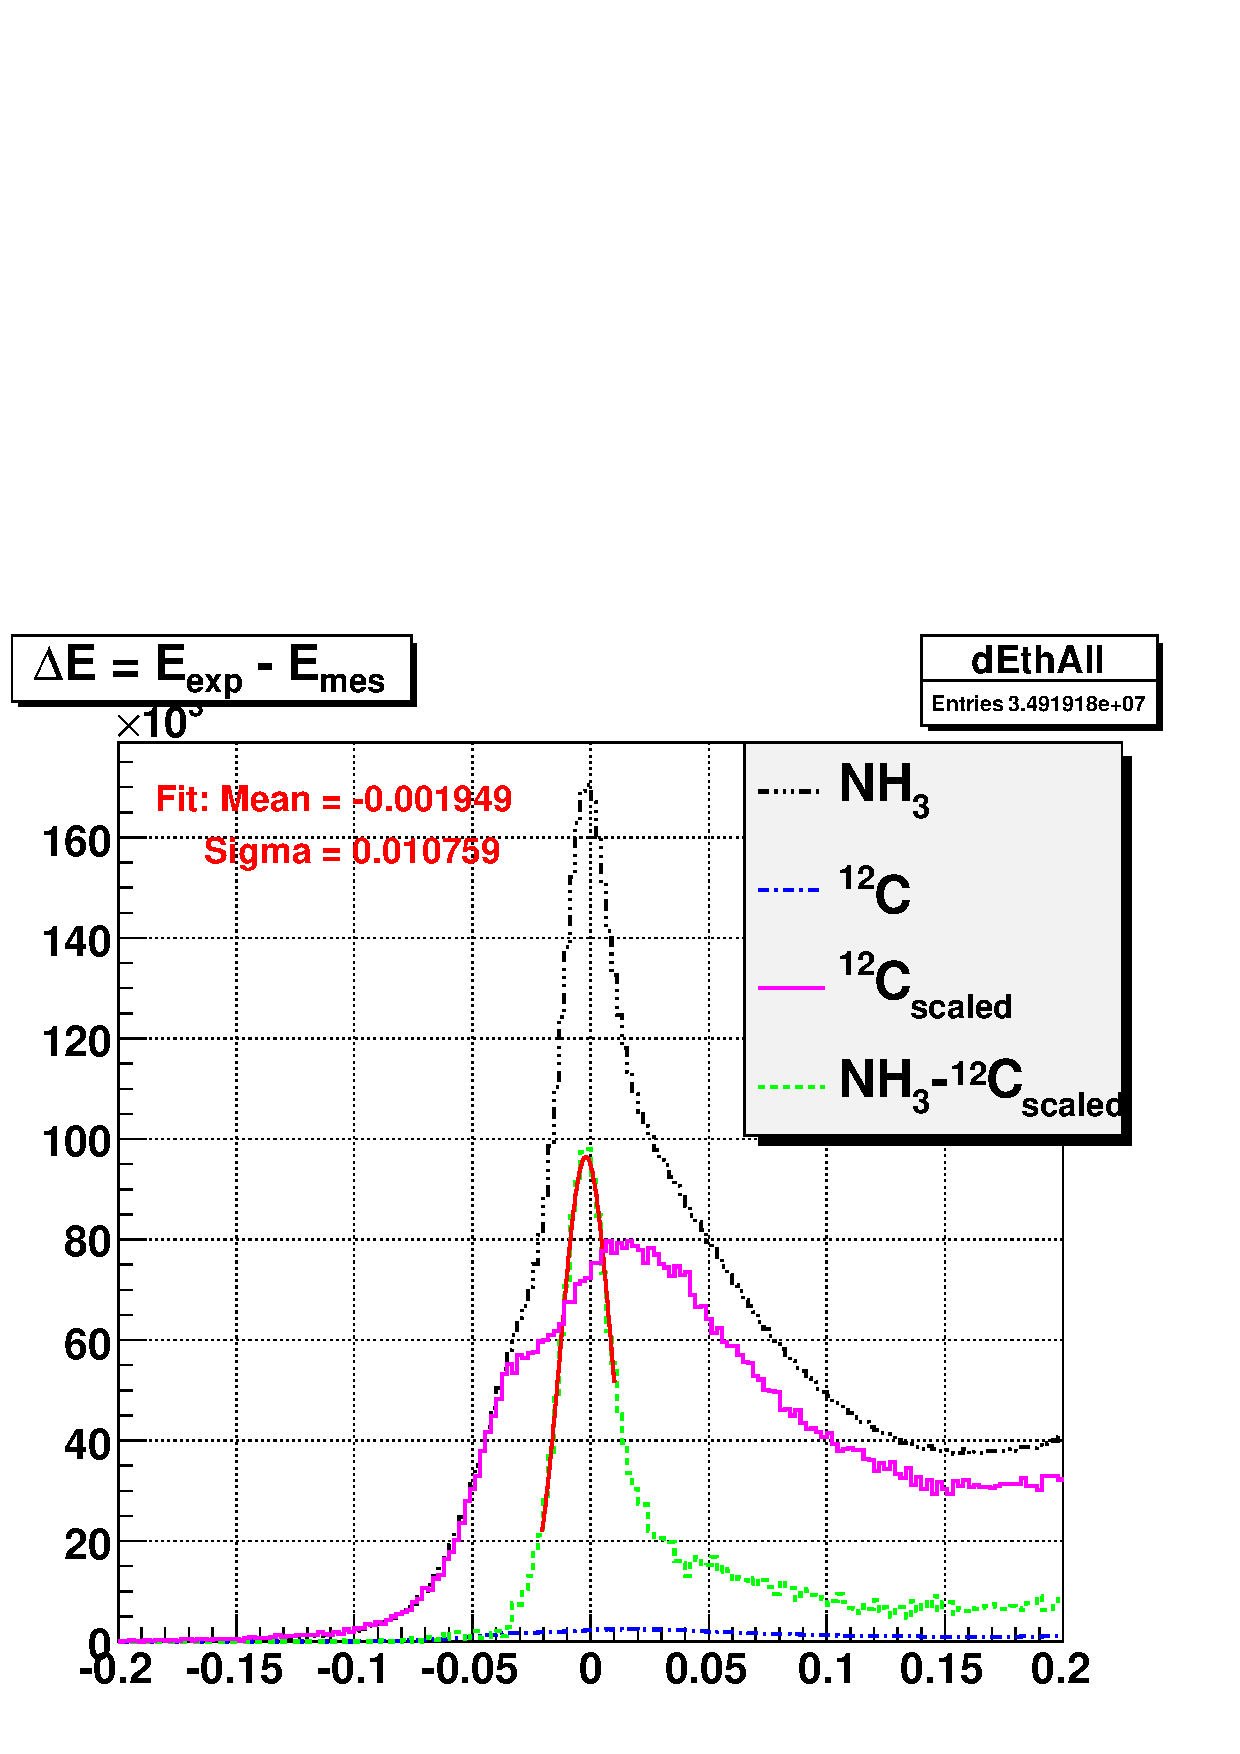
\includegraphics[width=0.8\textwidth]{figuresEG4/DcSmear/dE_elastProdEb3.png} 
  \caption[Background subtraction to get elastic peak]{Histograms illustrating the extraction of elastic peak for 2.3 GeV by using carbon-12 data for background removal from the total-cross section (all good electrons with $\theta>7$ used).}
  \label{fig:elNH3mC}
\end{figure}

%The following image is made using ~/Acceptance/SimStuffs/subtractHistos4xsDiff.C and enabling ``#define DRAW_EPS'' & ``#define USE_THETA_ALL''
\begin{figure}[h] %ht, htpb (p - float, b = bottom, h=? t = top)
\centering
  \leavevmode 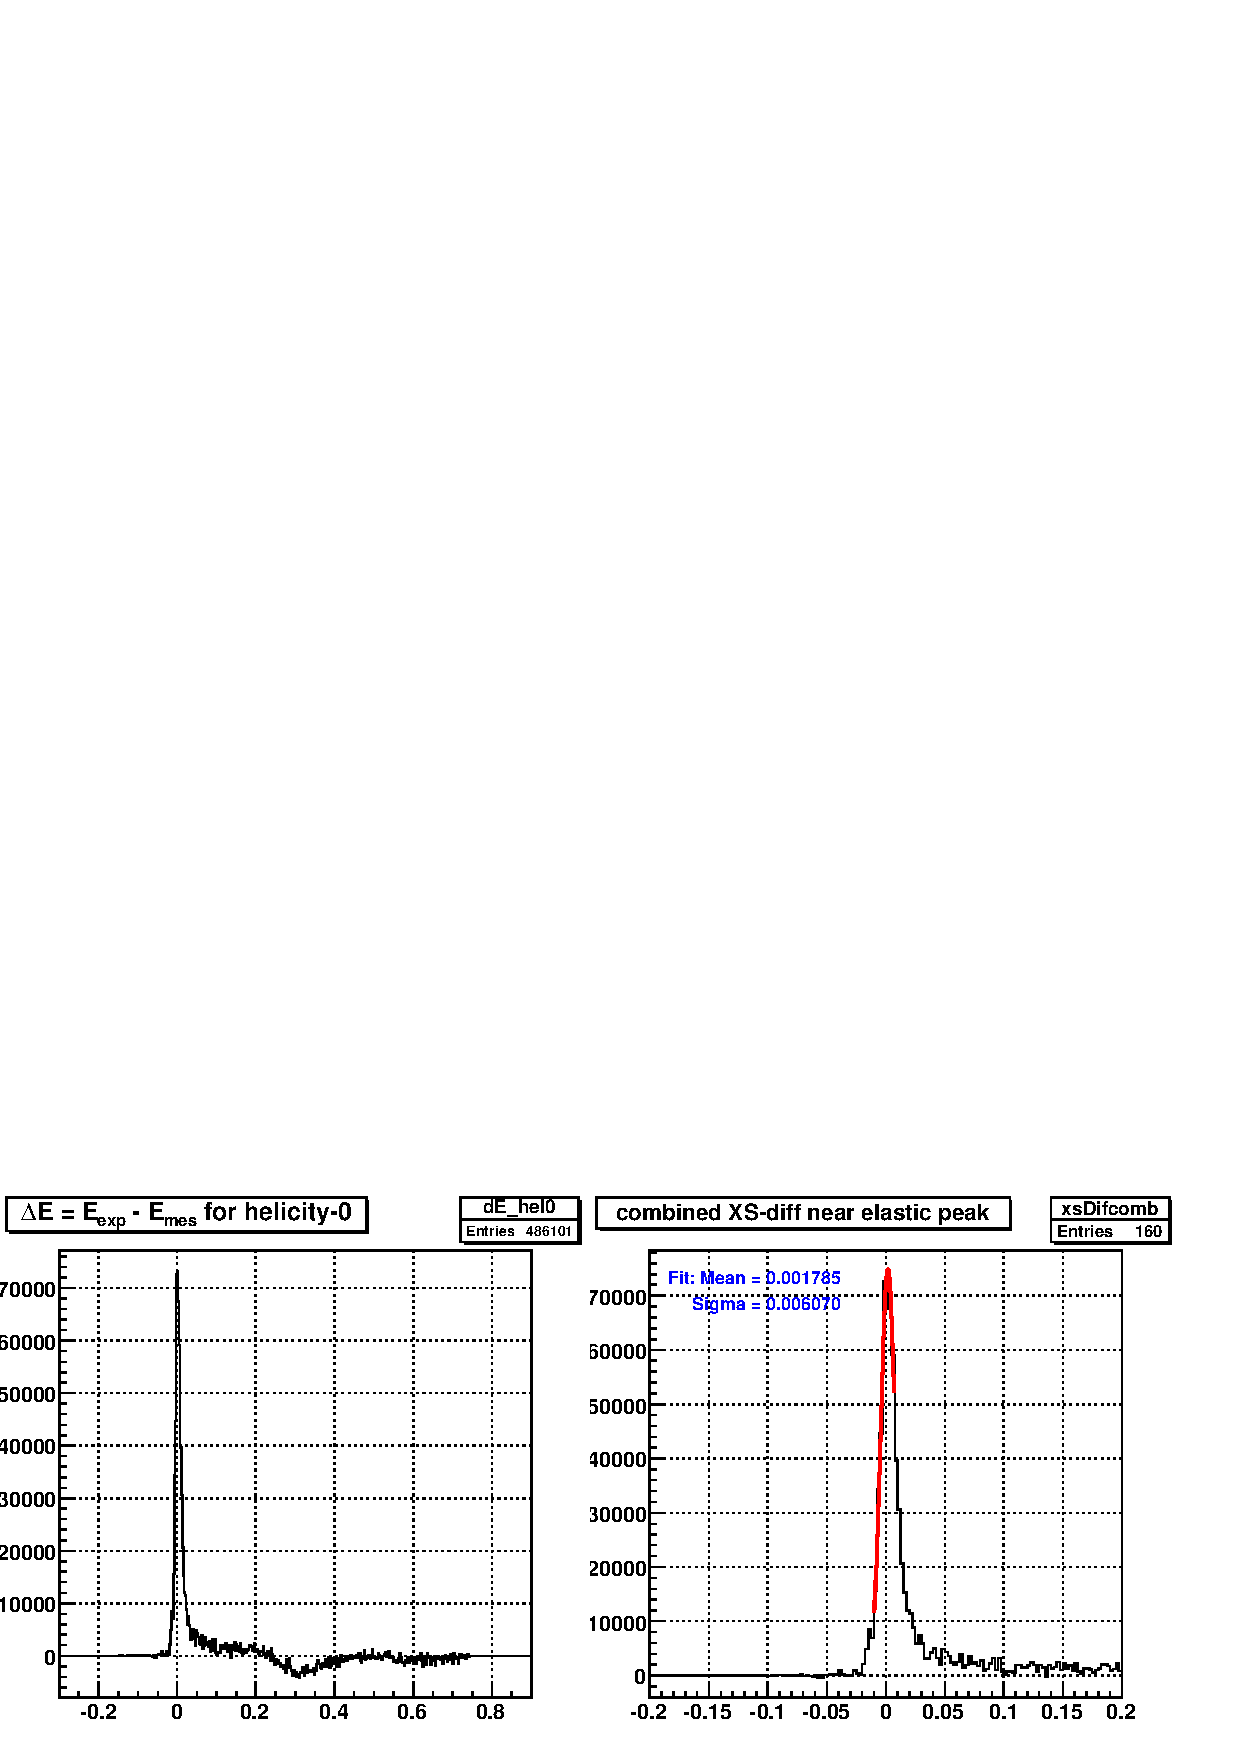
\includegraphics[width=1.0\textwidth]{figuresEG4/DcSmear/dE_elastXsDiffEb0Tgt11.png} 
  \caption[Cross-section difference]{Plots showing the cross-section difference for 2.3 GeV NH$_3$ target data with the right one zoomed in around the elastic region (all good electrons with $\theta>7$ used).}
  \label{fig:elXsDif}
\end{figure}

 %\\ %12/4/13 (Addressing Gabriel's concern)
 %\\
 



%\subsection{Comparing the width of the real CLAS data elastic peak and those from Simulation with different DC-smears.}
%The following two images are made using ~/Acceptance/SimStuffs/graphSigmaVsEb.C and enabling ``#define DRAW_EPS'' & ``#define USE_THETA_ALL''
Using the first of the two methods mentioned above, the real data resolutions were evaluated for three different %cases 
polar angle ($\theta$) cuts - 
all \th (in fact $\theta\ge7^o$), $\theta>15^o$, and $\theta>20^o$. The dependence of these experimental resolutions on the beam energy for these cases are 
shown together in the Fig. \ref{fig:sigsProd}, along with the resolution for the case ``all $\theta$'', but determined from the cross-section difference 
method. Likewise, as described above, the DC-smear dependence of the simulated resolution were determined separately for all these three cases of 
angle cuts, so that we could compare the experimental resolutions with the simulations correspondingly. One such comparison is illustrated in 
the figure \ref{fig:sigsProdSim}, where we show resolutions evaluated for the case of ``all \th'' - first two for the experimental data and the rest for 
the simulated data. 

    
     
 \begin{figure}[h] %ht, htpb (p - float, b = bottom, h=? t = top)
\centering
  \leavevmode \includegraphics[width=1.0\textwidth]{figuresEG4/DcSmear/graphSigmaVsEb_prodOnly.png} 
  \caption[$E_{beam}$ dependence of DC smearing (Experimental) ]{Graphs showing the dependence of width ($\sigma$) of the elastic peaks (from experimental data) on the beam energy (GeV).}
  \label{fig:sigsProd}
\end{figure}
    
 \begin{figure}[h] %ht, htpb (p - float, b = bottom, h=? t = top)
\centering
  \leavevmode 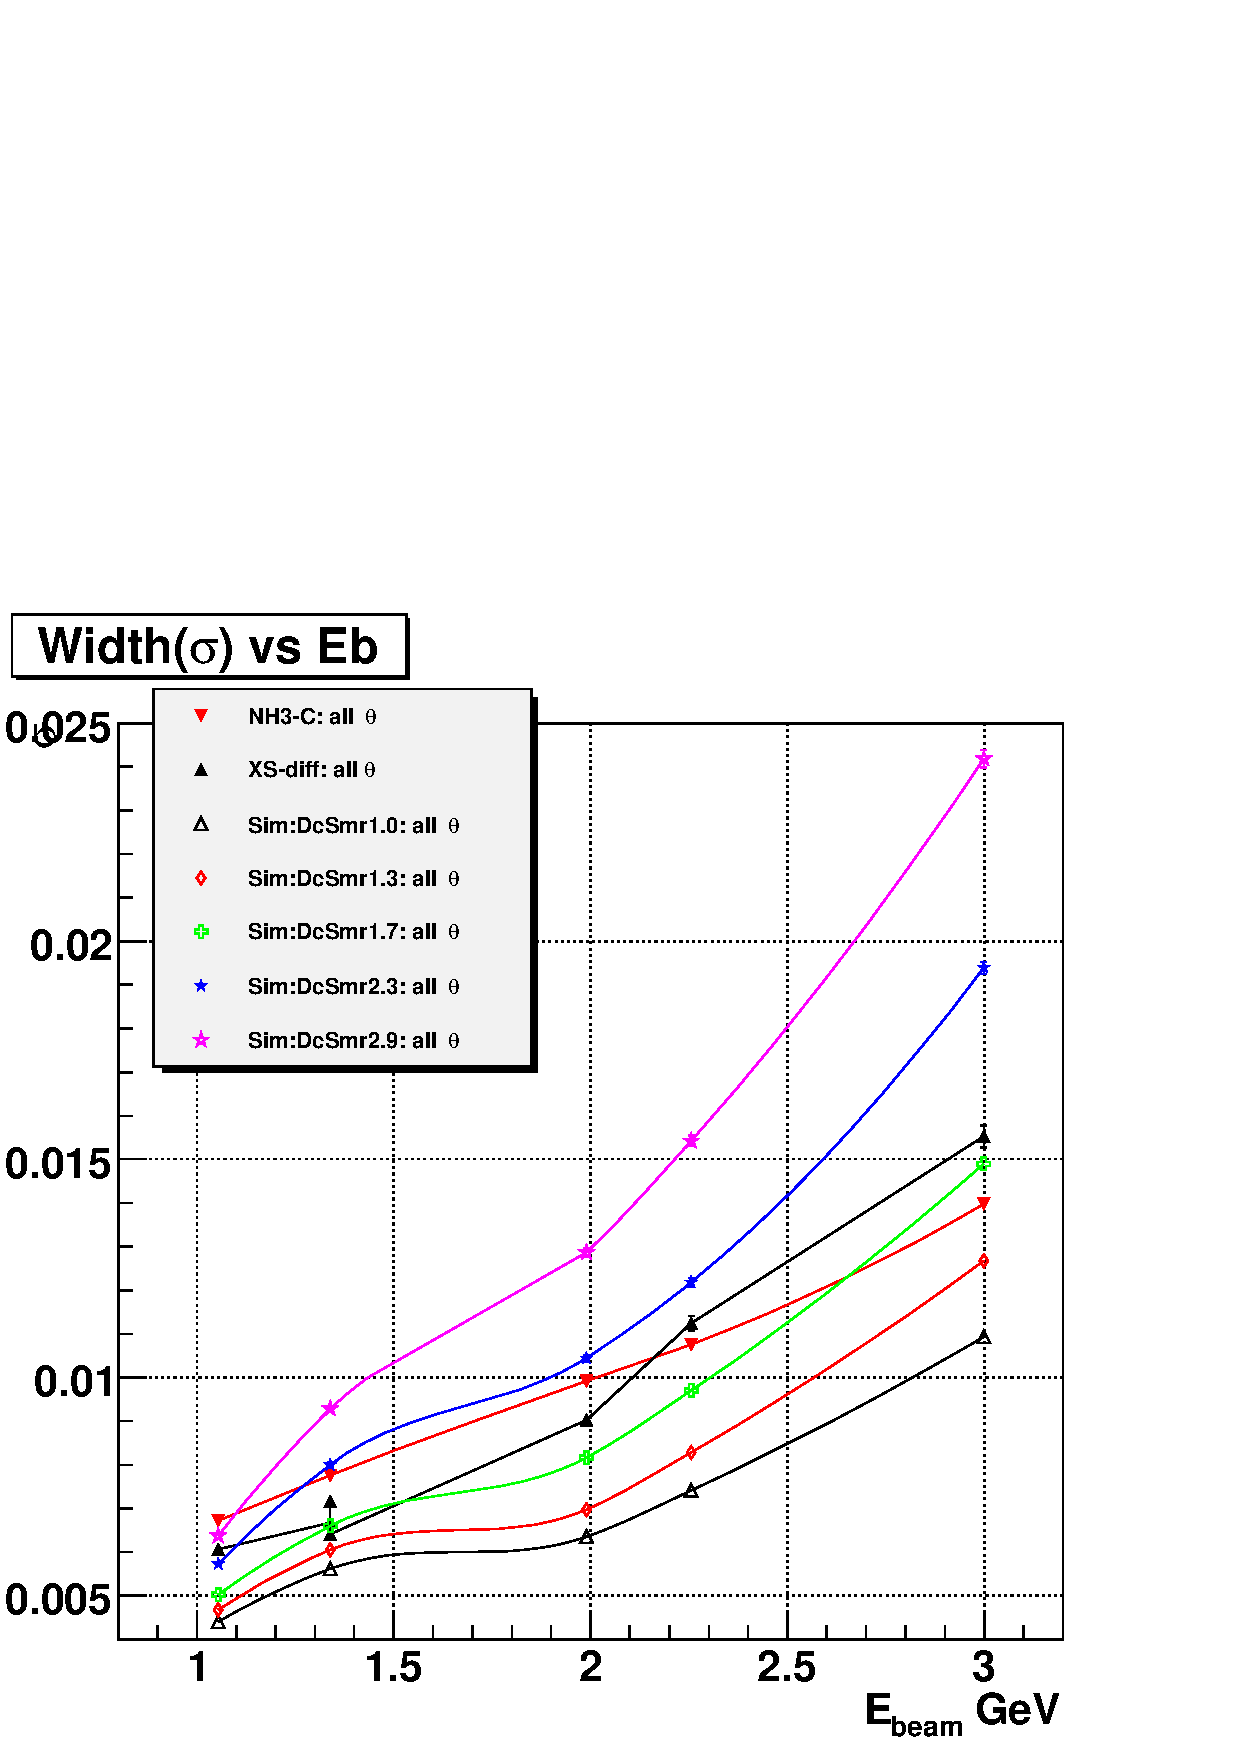
\includegraphics[width=1.0\textwidth]{figuresEG4/DcSmear/graphSigmaVsEb_SimThAll.png} 
  \caption[$E_{beam}$ dependence of DC smearing (Experimental) ]{Graphs showing the dependence of width ($\sigma$) of the elastic peaks (from both experimental and simulated data) on the beam energy (GeV).}
  \label{fig:sigsProdSim}
\end{figure}
    
     
     
Looking at Fig. \ref{fig:sigsProd}, it is obvious that the resolution is $\theta$-dependent as expected. %Remember resol = beta/sqrt(p_t), mom-cor
When the experimental and simulated resolutions are compared for the three different cases of $\theta$ cuts, we realize that the GPP asks for the 
\th dependent DC-smearing, which makes the simulation work very complicated with the current version of GPP. To simplify the situation, we decide to 
have a global (\th independent) value of DC-smearing (for a given beam energy) by comparing the experimental and simulated resolutions corresponding to 
the case of ``all \th'' cut. %That should be good enough for practical purposes. %xz:
%xz: "That should be good enough for practical purposes". Why?  Be careful to never make a statement without backing it up.
By taking into account the fact that there seems to be an inherent 
uncertainty in the measurement of the resolutions (evident from the discrepancy of the experimental resolutions determined from the two different methods)
and comparing the experimental and simulated results, the values as listed in Table. \ref{tab:dcSmears} are chosen for the DC-smearing scales for the GPP.


%\FloatBarrier  
% \FloatBarrier %http://tex.stackexchange.com/questions/9485/how-to-fix-table-position
%\begin{center}
\begin{table}[H]%[h] %[h!b!p!]
\centering
    \caption{DC-smearing scales determined for different beam energies.}
    \label{tab:dcSmears}
    \begin{tabular}{ | l | l | l | l | l | l |}
    \hline
    $E_{beam}$ (GeV) & 1.054  & 1.339 & 1.989 & 2.256 & 2.999 \\ \hline
    DC-smear         & 2.6    & 2.0   & 2.0   & 2.0   & 1.7 \\  \hline
    \end{tabular}
%    \caption{DC-smearing scales determined for different beam energies.}
%    \label{tab:dcSmears}
\end{table}
%\end{center}




\begin{comment} %==================My comments on the generated events==========Comments begin=== Sep 19, 2011
%The events were generated by using the Genova inherited mod_osip_bost (aka STEG) generator 
      subroutine smrad_proton(Es,theta,Ep,sig_el,sig_tot,sel,smin)
      common/material/TG
      sn2=(sin(theta/2.0))**2     Q2=4.0*Es*Ep*sn2       nu=Es-Ep
c-----input values
      Mp=0.93827        Z=1      A=1     E3=Es/(1.0+Es*(1.0-cos(theta))/Mp)
c-----elastic peak width==resolution
      dWp=0.001       delta_E=(dWp+dWp**2/(2.0*Mp))/(1.0+2.0*Es/Mp*sn2)/5.
c-----Target thickness
      t=0.0181              ! 0.6 cm NH3
      tiw=0.0079            ! 7.45 mm He
      tfw=0.0079            ! 7.45 mm He

      elra=0.0d+0       innn=0.0d+0       eltail=0.0d+0
c-----cross section
      if(Ep.gt.(E3-2.0*delta_E)) then
      varr=abs(nu-Q2/(2.0*Mp))
      jack=Es/E3
      elcor=elasrad_proton(Es,theta,t,delta_E,Z,A,tiw,tfw)                     ! cole smith program for radiative correction in the elastic region
      elra=sig_elastic_proton(Es,theta,Mp,Z)*elcor*peak_proton(varr,dWp)*jack
      
      innn=0.0d+0
      eltail=0.0d+0
      else
      elra=0.0d+0
      
      streg_tail=straggling_elasic_proton(Z,Mp,t,Es,Ep,theta,delta_E)           !But this is not added to anything so it's inconsequencial
      endif
            
      sel=elra+eltail
      smin=elra+innn+eltail
      return
      END


Comments:
There are two if blocks in the above chunk of the code:
     a) the ``if'' block which covers the elastic region
     b) the  ``else'' block which covers the rest of the region.
The else block has zero contribution to the value returned by the function because we set 'innn' and 'eltail' to zero and 'streg_tail' is not added to 
the sum to be returned.

As we see, the way I did is (being unsure how to turn off the effect of elcor (Cole smith's rad-corr)) leave the target widths t, tiw and tfw as they 
were (i.e. to non-zero values), and also leave the elcor factor alone, so that it would have some modulating effect on the remaining part of the product  
i.e. sig_elastic_proton(Es,theta,Mp,Z)*peak_proton(varr,dWp)*jack. Initially I thought I would give elcor an artificial value of 1.0 and that would 
probably turn off the effect. But, because of lack of confidence in that idea, I abandoned that idea and left it to modulate the elastic peak (may be 
the peak would come out more like a Gaussian, if I had done that). Even with that modulation, the generated events are within 3 MeV range and so the 
modulation would be insignificant. Another thought that came to my mind was that since this factor should have the effect of reducing the events in the 
elastic region to compensate for the radiative tail that we get beyond the elastic region, and since we're not simulating that part, there is no point 
in worrying about that reduction. If if the factor reduced the cross-section, the generator would produce the same number of events by running some extra 
mile to compensate for that reduction. 
\end{comment}  %=======================================Comments end
